\paragraph{Tijdsduur}
\begin{figure}[H]
    \centering
    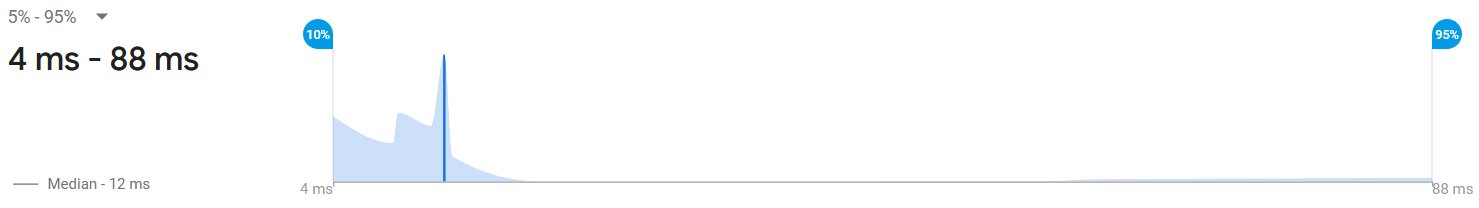
\includegraphics[height=0.1\textheight]{notificatiesDuratieNative.png}
    \caption{Overzicht tijdsduur aanmaken notificaties bij Android.}
\end{figure}
Tijdens het meten van de duur voor het aanmaken van een notificatie, is er 
10 keer een notificatie aangemaakt. Na 10 keer een notificatie aan te maken is er  
een gemiddelde duur van 12ms en met een minimum en 
maximum van 4ms en 88ms.

\paragraph{CPU \& geheugen}
\begin{figure}[H]
    \centering
    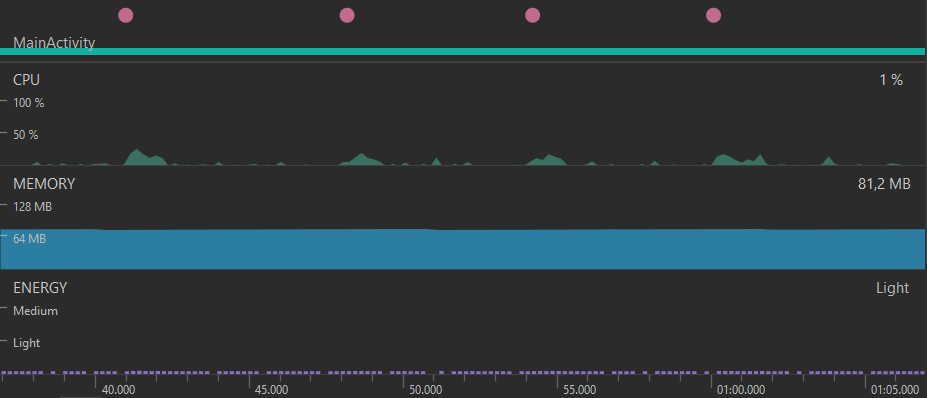
\includegraphics[height=0.25\textheight]{notificatiesPerformantieNative.png}
    \caption{Overzicht CPU en geheugen gebruik tijdens aanmaken notificaties bij Android.}
\end{figure}
Op de grafiek is te zien dat het CPU gebruik van de applicatie wanneer deze inactief is, rond de 4\% ligt. 
Het is ook duidelijk zichtbaar wanneer een notificatie wordt aangemaakt. De piek van het CPU gebruik lag 
gemiddeld op 21\% en schommelde tussen de 19\% en 27\%. Het geheugen blijft in tegenstelling met de CPU 
wanneer de applicatie inactief en actief is, rond de 81MB hangen, met verschillen van maximum 2-3MB. Er is geen 
merkbaar verschil in het geheugen wanneer een notificatie wordt aangemaakt.
  